\chapter{Feature Selection}

\newthought{Sometimes, measuring features is expensive} or training a model needs to be fast yet accurate. It can also happen that a large number of features make the model difficult to interpret. Hence it is handy to know which features are actually important for the model and which are redundant. And in order to determine which are those features, we use a process called feature scoring.

\begin{wrapfigure}{o}{0.6\textwidth}
    \vspace{-0.5cm}
    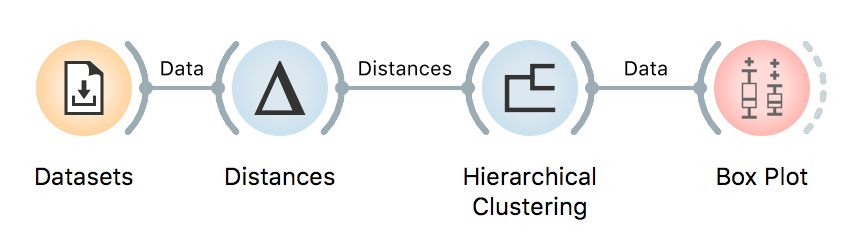
\includegraphics[scale=0.4]{workflow.png}
\end{wrapfigure}

There are several scoring methods, some of which are univariate (they look at the relationship between a single feature and the target variable), some are multivariate (they can consider multiple features), and some are model-based (they use models to estimate feature importance). 

One such scoring technique is called \textit{information gain}. Let us consider feature X and the target variable Y. Information gain is a univariate method measuring the amount of information gained Y knowing the value of X.

%box plot
A similar method is \textit{Gini decrease}, which also measures decrease in impurity after observing the variable (X). They both favor multilabel features, because they tend to split the data more resulting in purer subsets. This was the reason behind conception of \textit{Relief} (later improved to ReliefF), which handles multilabel and numeric data better. It also has one important advantage - it is a multivariate method, which means it can handle the so-called XOR problems\marginnote{An XOR problem is a problem where the final class would be a result of }

\begin{figure}[h]
    \centering
    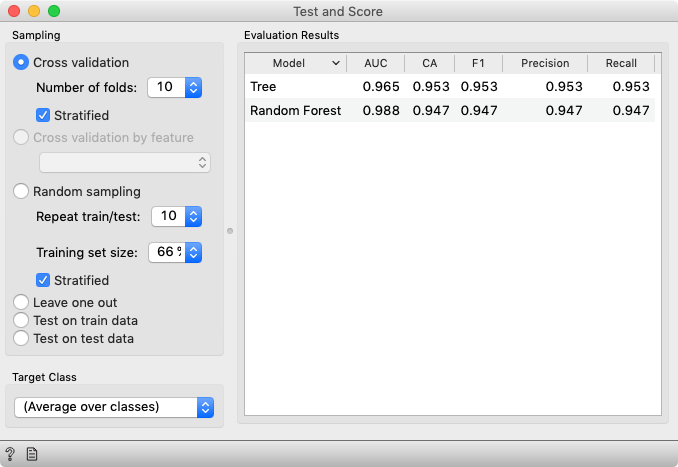
\includegraphics[scale=0.4]{test_and_score.png}
    \caption{Cross validation splits the data sets into, say, 10 different non-overlapping subsets we call folds. In each iteration, one fold will be used for testing, while the data from all other folds will be used for training. In this way, each data instance will be used for testing exactly once.}
\end{figure}
